%-------------------------------------------------------

\documentclass{article}
\usepackage{anysize}

\marginsize{2cm}{2cm}{1cm}{2cm}
\usepackage{algorithm}

\usepackage{algorithmic}

\usepackage{multirow}

\usepackage{amsmath}


\usepackage{xcolor}

\DeclareMathOperator*{\argmin}{argmin}

\renewcommand{\algorithmicrequire}{\textbf{Input:}}

\renewcommand{\algorithmicensure}{\textbf{Output:}}
\renewcommand{\part}[1] {\vspace{.10in} {\bf (#1)}}
\newcommand{\myname}{Chenwei Xie A53091839,  Jiaixiang Chen A53100265, Yue Wang A53102167}

\usepackage{graphics}

\usepackage{graphicx}

\usepackage{epsfig}

\begin{document}

\thispagestyle{plain}
\begin{center}                  % Center the following lines
{\Large CSE231 Project 1 } \\
\myname \\
\end{center}

\section{Overview}

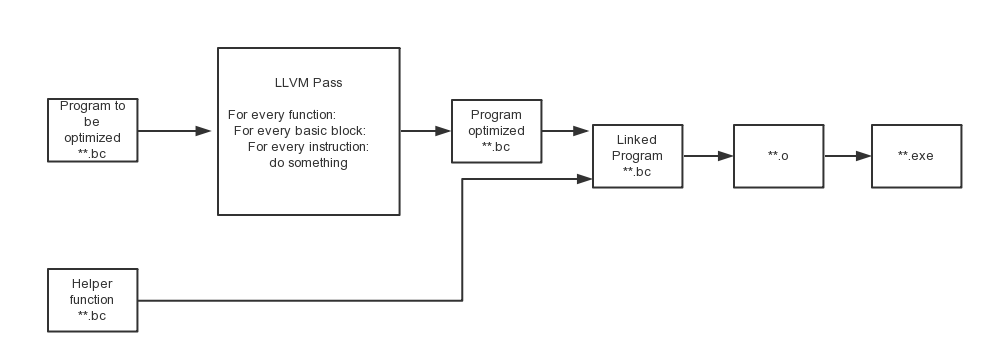
\includegraphics[height=4.5cm]{graph.png}\\

\section{Collecting Static Instruction Counts}

\part{1} Algorithm
	

This section mainly consists of 2 procedures: first is to gather information about all instructions found, and this should be done during the procedure of traversing all instructions. And second is to print out all instructions and their counts after traversing all instructions.For storing all information, we used a map to keep track of names of all instructions and how many found.

Since we need to analyze a program, we need to traversing all modules, so we implemented our pass under ModulePass class, and override the function runOnModule. In the function runOnModule, we iterated all functions, all basic blocks and all instructions. getOpcodeName() is used to get instruction names of every instructions. So for every instructions, we first find if it is in our map, then to decide whether to add it to map or increase the number stored.
	
\part{2}Challenge
	

As this is the first problem in this project, it isn't so hard as other problems, and the major difficulty comes from the use of LLVM, since it is the first llvm pass we write, there are some concepts like module, function and basicblock that we are not familiar with.




\section{Collecting Dynamic Instruction Counts}

\part{1}Algorithm:

A basic block is a single-entry, single-exit section of code. So whether the program is running or not, the static analysis for a basic block is the same with the dynamic analysis for this block. The idea is to calculate the statistic for the basic block statically when the LLVM Pass optimize the target program and in the end of each basic block, the LLVM Pass we implement will insert a function call to a global function $merge$. When the program is running, every time the program comes across the inserted point, the program will call $merge$ and the function will combine the statistic of this basic block to a global map. So probably a basic block can run several time, which means the statistic of this basic block will be merged into global map several time. Also in the termination of the program, we need to output the result. So when the LLVM Pass optimize the program, it also find the $main$ function and then find the $return$ statement and just before the $return$ statement, LLVM Pass inserts a function call to $print$ which can output the statistic result of this program. The two function $print$ and $merge$ are put in a file called merge.cpp.

At high level, one program and merge.cpp are passed to clang, and clang generates their LLVM IR. And then, the LLVM Pass will optimize the $program$'$s$ LLVM IR. And then the compiler will link the modified program LLVM IR and merge LLVM IR together and then compile them into the executable.


\part{2} Challenge:

The challenge here is the almost the same with what we come across in part 3. The first thing is how to pass the parameter when inserting a function. Passing a string is hard, so we pass a integer(opcode) and the using LLVM's getopcodename to get the real name of the instruction. Second thing is how to find a appropriate insertion point. However, in this case, we find out the insertion point in a basic block doesn't matter.


\section{Profiling Branch Bias}


\part{1} Algorithm:

We have there pieces of inserting functions here, their function name and usage are listed as below:
Collecting all function names in this module,
Handling all branch instruction for each function in this module,
Printing the result.

Our algorithm to insert the code is shown as below: First insert code in each basic block to collect all function names, then for each instruction in basic, we judge whether it is a $ret$ instruction and it is in $main$ function or it is a conditional $br$ instruction. If it is a $ret$ instruction and in $main$ function, then insert the $printing$ $result$ function here. Or if it is a $br$ instruction, then we insert a function call to handle this branch. The 3 inserted functions will do the following things: $Printing$ $the$ $result$ obviously accepts no parameter and output the result. $Collecting$ $all$ $function$ $names$ $in$ $this$ $module$ accepts $char *$ parameter which is the name of the function and it store the function name(In case some functions have no branch instruction). $Handling$ $all$ $branch$ $instruction$ $for$ $each$ $function$ $in$ $this$ $module$ will accepts two parameters, namely $function$ $name$ and $branch$ $condition$, if the $branch$ $condition$ is true, it will increase the taken number of the function. And it also increases the total branch number in this function.



API used:
isConditional(),
getOperand(1),
getName()


\part{2} Challenge:

The first challenge is how to judge if a $br$ instruction execute or not.
We try three different ways to solve the problems.
	1. Get the value of $br$ instruction directly
		In llvm::BranchInst, we find there is a member function called getCondition(). At first, we think that it will return a value to tell us whether the condition is true or false. Since the return type is Value*, we try to cast it to a integer and the get the value, however, after we try this and search the internet, we find this function actually return the expression of $br$ instruction, so we give up this way and try our second solution.
	2. Evaluate the value of expression in $br$
		Since we now have the expression of $br$  instruction by using getCondition(), we want to evaluate this expression to know if the instruction will be taken or not. We find there is a class called llvm::MCExpr and it has a function called evaluateAsAbsolute() that could get the value. So, we try to cast out expression to it and want to get the value. We failed that llvm tells us that this two class can not be cast.
	3. Store the label of $br$ and count it later
		We think that we could first store all possible basicblock that $br$ instruction will go to, and when run the program, we could search if one running basicblock is from a $br$ instruction. So, we use two loop here, one to store and one to count the actually taken basic blocks. However, then we found a situation where this will fail, that is, when a branch calls a function, then the branch will be recorded in original block, but the taken will be recorded in the new block.
    4. Turn back to get the value of $br$.
        Then when we look back, we found that though the result of getCondition() is a Value* and we do get a string value containing the condition instruction, but then we found that by passing it as a boolean value, we can still get the condition value in the running time. So this is the final solution we got.

Another challenge comes from how to passing string values to functions to be inserted. At first we want to use getName() method the of function iterator to get the function name and then pass it to the function counting branches. However, string is not a valid type to be passed using $llvm::Value*$, since there is no such a type called stringTy in llvm::Value. Then we tried to pass a pointer standing for a C type string as argument, but the idea didn't work either, since the string in the pass file is not same as the string in the file to be combined with the target code file, so passing such a pointer will only lead to segment fault at last. Finally we found the solution, to use global variables to store strings. And to get the instructions needed to insert global variables, we write a simple cpp file containing only a definition of global string and then compile it to llvm instruction and then reconstruct it, to find how llvm store global variables.



\section{Result Analysis}


Here, we want to analyze the benchmark hadamard. From the static result, there are only 212 instructions totally, but as for the dynamic result, the program executes 37881 instructions totally, which means in average, every instruction executes 178 times. So if we can reduce the number of instructions of this program, maybe the running time will drop significantly. And as for the branch statistic, the branch is very likely to be taken in this program. Which means if we can optimize this program by predicting the branch taken or not, it's sensible to predict the branch being taken.\\


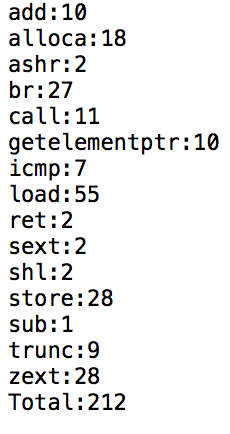
\includegraphics[height=2cm]{static.png}
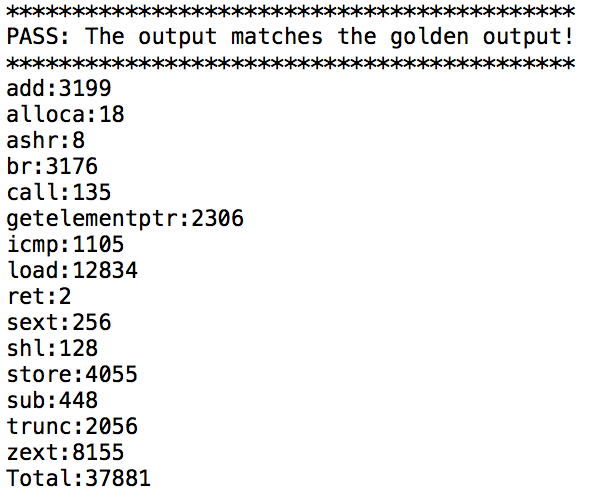
\includegraphics[height=2cm]{dynamic.png}
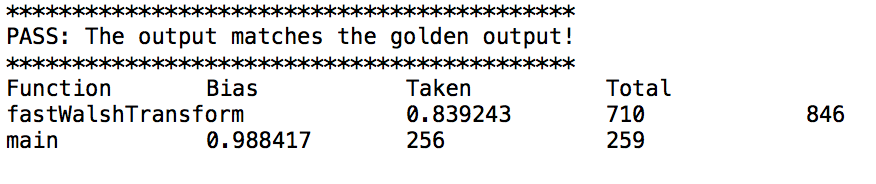
\includegraphics[height=2cm]{branch.png}\\
\section{Pseudo Code}

\begin{algorithm}[htb]
\caption{ Collecting Static Instruction Counts }
\begin{algorithmic}
\FOR{each function in the module}
    \FOR{each basicblock in the function}
		\FOR{each instruction in the basicblock}
			\STATE increase the number of corresponding instruction
		\ENDFOR
	\ENDFOR
\ENDFOR
\end{algorithmic}
\end{algorithm}



\begin{algorithm}[htb]
\caption{ Collecting Dynamic Instruction Counts }
\begin{algorithmic}
\FOR{each function in the module}
    \FOR{each basicblock in the function}
		\FOR{each instruction in the basicblock}
            \IF {the instruction is $return$ and the function is $main$}
                \STATE insert a function call to $print$ the statistic of the program
			\ENDIF
			\STATE increase the number of corresponding instruction
		\ENDFOR
		\STATE insert a function call to $merge$ the statistic into global map in the end of each basic block
	\ENDFOR
\ENDFOR
\end{algorithmic}
\end{algorithm}


\begin{algorithm}[htb]
\caption{ Profiling Branch Bias}
\begin{algorithmic}
\FOR {function in Module}
    \FOR {basicblock in function}
        \STATE insert function\_name function
        \FOR {instruction in basicblock}
            \IF {instruction is ret and it is in main function}
                \STATE insert print\_result function
            \ENDIF
            \IF {instruction is conditional br}
                \STATE getcondition value
                \STATE insert count\_branch function
            \ENDIF
        \ENDFOR
    \ENDFOR
\ENDFOR

\end{algorithmic}
\end{algorithm}


\end{document} 